\documentclass[a4paper,10pt]{article}
\usepackage[margin=1in]{geometry}
\usepackage{polski}
\usepackage[utf8x]{inputenc}
\usepackage[unicode]{hyperref}
\usepackage{amssymb}
\usepackage{xifthen}
\usepackage[fleqn]{amsmath}
\usepackage{todonotes}
\usepackage{graphicx}
\usepackage{float}
\usepackage{fullpage}
\usepackage{epstopdf}
\usepackage{multirow}
\usepackage{subfig}
\usepackage[europeanresistors,americaninductors]{circuitikz}
\usetikzlibrary{patterns}
\newcommand{\withtodo}{0}


\def\arraystretch{1.2}


\begin{document}

\begin{table}
  \centering
  \def\arraystretch{1.5}
    \begin{tabular}{|l|l|l|l|} \hline
    Wydział:           & \multicolumn{2}{l|}{Dzień:Poniedziałek 14-17}    &Zespół:  \\
    Fizyki             &    \multicolumn{2}{l|}{Data: 08.05.2017}         &8             \\\hline
    Imiona i nazwiska: &Ocena z przygotowania:  &Ocena ze sprawozdania:   &Ocena końcowa: \\
    Marta Pogorzelska  &                        &                         &                \\
    Paulina Marikin    &                        &                         &\\\hline
    \multicolumn{2}{|l|}{Prowadzący:                 } &\multicolumn{2}{l|}{Podpis:             }  \\\hline
  \end{tabular}
\end{table}

\title{Ćwiczenie 34:\\Wyznaczanie dyspersji optycznej pryzmatu metodą kąta najmniejszego odchylenia}

\section{Cel badań}
Celem doświadczenia było wyznaczenie krzywej dyspersji danego pryzmatu prostego.

\section{Wstęp teoretyczny}
Dyspersja jest własnością optyczną materiałów zgodnie z którą, prędkość fali elektromagnetycznej poruszającej się przez dany materiał jest zależna od jej częstotliwości. Ponieważ współczynnik załamania danego ośrodka jest zależny od tejże prędkości, on także będzie się zmieniał w zależności od częstotliwości fali.
\begin{equation}
n(\nu) = \frac{c}{v(\nu)}
\end{equation}
, gdzie n - współczynnik załamania światła, c - prędkość światła w próżni, v - prędkość światła w danym ośrodku, $\nu$ - częstotliwość fali

W przypadku światła białego, zawierającego fale o różnych częstotliwościach, zostanie ono rozszczepione na pojedyńcze wiązki, załamujące się pod innym kątem.

Wiązka światła monochromatycznego przy przechodzeniu przez pryzmat odchyla się o kąt $\varepsilon$, zawarty między pierwotnym jej biegiem a wiązką załamaną. 
\begin{figure} [H]
  \centering
  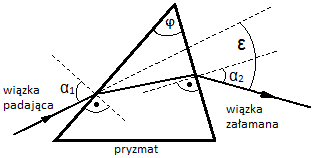
\includegraphics[width=0.5\textwidth]{./epsilon.png}
  \caption{Kąt odchylenia $\varepsilon$ wiązki światła przy przechodzeniu przez pryzmat.}
  \label{}
\end{figure}

Kąt odchylenia $\varepsilon$ zależy m.in. on od kąta padania $\alpha$ i jest najmniejszy w sytuacji, gdy kąt padania $\alpha_1$ i kąt wyjścia $\alpha_2$ są równe. Jest to tzw. "przebieg symetryczny", dla którego, w oparciu o prawo Snelliusa, zachodzi równość:
\begin{equation}
n = \frac{\sin \frac{\varepsilon_{min}+\varphi}{2}}{\sin \frac{\varphi}{2}}
\end{equation}
\begin{figure} [H]
  \centering
  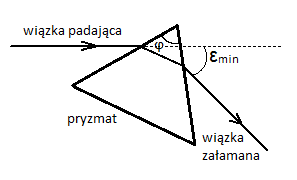
\includegraphics{./epsilon_min.png}
  \caption{Kąt najmniejszego odchylenia $\varepsilon_{min}$ dla tzw. przebiegu symetrycznego.}
  \label{}
\end{figure}

\section{Opis układu i metody pomiarowej}
Aparatura pomiarowa
\begin{itemize}
  \item lampa sodowa
  \item lampa neonowa
  \item spektrometr
\end{itemize}
\subsection{Kąt łamiący pryzmatu}
Najpierw należało wyznaczyć kąt łamiący danego pryzmatu. W tym celu włączono lampę sodową i postawiono ją tak, by światło padało bezpośrednio przez kolimator spektrometru. Pryzmat ustawiono na stoliku tak, by kąt łamiący znajdował się naprzeciw kolimatora. 
\begin{figure} [H]
  \centering
  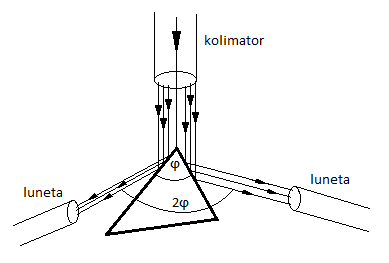
\includegraphics[width=0.5\textwidth]{./phi.png}
  \caption{Kąt łamiący pryzmatu}
  \label{}
\end{figure}
Następnie, obserwując %i tu nie wiem światło? obraz światła?
przez lunetę, należało wyregulować jego ostrość oraz szerokość obrazu szczeliny tak, by była możliwe jak najwęższa. Następnie odszukujemy wiązkę odbitą od jednej i drugiej ścianki pryzmatu i odczytujemy przy pomocy kątomierza ich położenie kątowe. Kąt łamiący $\varphi$ wyznaczamy ze wzoru:
\begin{equation}
\varphi = \frac{a_1 - a_2}{2}
\end{equation}
, gdzie $a_1, a_2$ - położenie kątowe lunety dla każdej z odbitych wiązek

\subsection{Kąt najmniejszego odchylenia}
Kolejnym pomiarem potrzebnym w doświadczeniu był pomiar kąta najmniejszego odchylenia. Ustawiamy pryzmat tak, by wiązka światła padała na jedną ze ścianek i wyszukujemy lunetą wiązki załamanej. Następnie manipulując stolikiem zmieniamy kąt padania, jednocześnie śledząc położenie wiązki przy pomocy lunety. Wiązka przesuwa się w prawo, by w pewnym momencie zatrzymać się i przy dalszym obrocie stolika zawrócić. Punkt zwrotny wyznacza położenie kolimatora i lunety, dla których kąt odchylenia $\varepsilon$ jest najmniejszy. (patrz rys.2)

\subsection{Pomiary właściwe}
Dla wyznaczonego kąta najmniejszego odchylenia odnajdujemy wiązki żółtą i zieloną i odczytujemy dla nich położenie kątowe lunety. Następnie, przy niezmienianiu położenia stolika, wyłączamy lampę sodową, odstawiwamy ją, włączamy lampę neonową i podstawiamy ją tak, by światło padało przez kolimator. Dla wciąż tego samego kąta najmniejszeg odchylenia wykonujemy analogicznie pomiary dla lampy neonowej. Dla kilku najjaśniejszych linii barw spisujemy położenie kątowe lunety.

\section{Wyniki pomiarów}
Kąt łamiący pryzmatu: $60^\circ$
\\Kąt zerowy: $45^\circ 30'$
\subsection{Pomiary dla sodu}
\begin{itemize}
  \item żółty 589nm $346^\circ 50'$ %589nm
  \item zielony (dlugość fali) $145^\circ 30'$ %568nm
\end{itemize}
\subsection{Pomiary dla neonu}
\begin{tabular}{lrrr}
{} &  $\lambda[nm]$ &  $\alpha[^\circ]$ &  $\alpha[']$ \\
0  &         654 &          348 &          18 \\
1  &         651 &          348 &          10 \\
2  &         641 &          348 &           0 \\
3  &         614 &          347 &          46 \\
4  &         610 &          347 &          40 \\
5  &         603 &          347 &          26 \\
6  &         591 &          347 &          10 \\
7  &         588 &          347 &           0 \\
8  &         540 &          346 &          20 \\
9  &         534 &          346 &          10 \\
10 &         470 &          345 &          48 \\
11 &         454 &          344 &          44 \\
\end{tabular}

\section{Analiza pomiarów}
%Do wykresu dorobię jeszcze dopasowaną krzywą i zrzutuję nań pomiary z sodu i naniosę niepewności
\begin{figure} [H]
  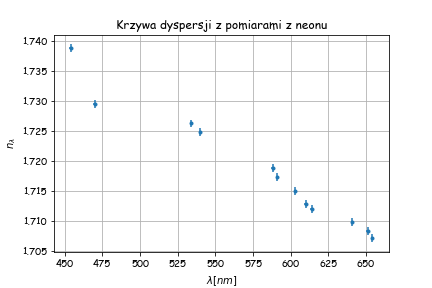
\includegraphics{./dyspersja.png}
  \caption{}
  \label{}
\end{figure}

\section{Analiza niepewności}
Za niepewność pomiaru wzięto:
\begin{equation}
  \Delta \alpha = \sqrt{(\frac{\Delta_k}{3})^2+(\frac{\Delta_o}{3})^2}
\end{equation}
gdzie $\Delta_k$ - podziałka kątomierza: $2'$, a $\Delta_o$ - niepewność eksperymentatora: $2'$.\\
\\Dalsze niepewności wyliczano metodą propagacji niepewności:
\begin{itemize}
  \item Kąt łamiący pryzmatu
  \begin{equation}
    \Delta \varphi = \sqrt{(\frac{\Delta \alpha_L}{2})^2+(\frac{\Delta \alpha_P}{2})^2}
  \end{equation}
  \item Kąt najmniejszego odchylenia
  \begin{equation}
    \Delta \varepsilon_{min} = \sqrt{(\Delta \alpha)^2+(\Delta \alpha_0)^2}
  \end{equation}
  \item Wspołczynnik załamania
  \begin{equation}
    \Delta n = \sqrt{(\Delta \varphi \frac{\sin{\left (\frac{\varepsilon_{min}}{2} \right )}}{\cos{\left (\varphi \right )} - 1})^2+
    (\Delta \varepsilon \frac{\cos{\left (\frac{\varepsilon_{min}}{2} + \frac{\varphi}{2} \right )}}{2 \sin{\left (\frac{\varphi}{2} \right )}})^2}
  \end{equation}
\end{itemize}

\section{Wnioski}


\end{document}
